\documentclass[a4paper,12pt,oneside]{scrreprt}
	\usepackage[utf8]{inputenc}
	\usepackage{graphicx}
	\usepackage{amssymb}
	\usepackage{setspace}
	\usepackage{amsmath}
	\usepackage{hyperref}
	\onehalfspacing % das ist der 1,5 zeilige abstand!!!
	\usepackage{geometry}
	\geometry{left=2.5cm,right=2.5cm,top=2.5cm,bottom=2.5cm}
	\usepackage{listings}
	\usepackage{color}
	\definecolor{mygray}{rgb}{0.4,0.4,0.4}
	\definecolor{mygreen}{rgb}{0,0.8,0.6}
	\definecolor{myorange}{rgb}{1.0,0.4,0}
	\lstset {
			basicstyle=\footnotesize\sffamily\color{black},
			commentstyle=\color{mygray},
			frame=single,
			numbers=left,
			numbersep=5pt,
			numberstyle=\tiny\color{mygray},
			keywordstyle=\color{mygreen},
			showspaces=false,
			showstringspaces=false,
			stringstyle=\color{myorange},
			tabsize=2
	}

\title{ Registermaschinenentwurf Py Register Machine \[design01\]}
\author{Daniel Knüttel}
\date{11.12.2015}


\begin{document}

\maketitle
\tableofcontents

\chapter{Abstract}

Registermaschinen sind ein interressantes informatisches Rechenmodell, sowie eine hervorragende Möglichkeit, um
hardwarenahes Programmieren zu lernen. In diesem Dokument sollen die grundliegenden Theorien sowie Entwürfe nähergebracht werden.

\part{Registermaschinenentwurf Py Register Machine}


\chapter{Begriffe}
\section{Registermaschine}

Eine Registermaschine beschreibt ein informatisches Rechenmodell: Sie hat mehrere Zustände ( mindestens 2 ) 
und kann diese ändern, den Zustand wechseln. Dabei spricht man von einer Transition.

Diese Zustände werden in der Registermaschine durch Speicherzellen repräsentiert, je nach Anwendungszweck bzw. Entwurf werden unterschiedliche Speicherzellen genutzt.

Dies lässt sich auf die Quintessenz der Registermaschine zusammenfassen: \textit{Die Registermaschine ist ein sich selbst modifizierender Speicher.}

\section{Transition}

Ändert eine Registermaschine ihren Zustand, so spricht man von einer Transition, \textbf{jeder Befehl}, den eine Registermaschine ausführt ist eine Transition.

\section{Endlichkeit}

Eine Registermaschine ist ein Endlicher Automat. Diese Endlichkeit bezieht sich allerdings nicht, darauf, dass die Registermaschine endlich lange ihren Zustand wechselt, sondern darauf, dass sie eine \textit{endliche Anzahl an Zuständen} besitzt.

Die wohl einfachste Registermaschine ist ein Zähler ( \ref{fig:zaehler} ): er kann nur einen Befehl ausführen, dieser erhöht die einzige Speicherstelle. Diese Registermaschine hat eine endliche Zahl an Zuständen ( die Breite der Speicherstelle ), aber eine ( theoretisch ) unendliche Laufzeit.

\begin{figure}
\centering
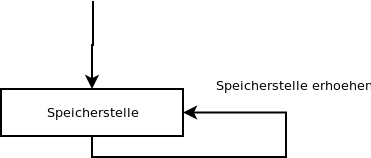
\includegraphics[width=300pt]{zaehler.png}
\caption[Flussdiagramm Zähler]{Flussdiagramm eines Zählers: ein endlicher Automat}
\label{fig:zaehler}
\end{figure}

Gehen wir von einem Zähler mit der Breite 4 bit aus, so ergeben sich die folgenden Zustände:

\begin{lstlisting}[frame=single]
binaer decimal
0000 = 0
0001 = 1
0010 = 2
0011 = 3
0100 = 4
0101 = 5
0110 = 6
0111 = 7
1000 = 8
1001 = 9
1010 = 10
1011 = 11
1100 = 12
1101 = 13
1110 = 14
1111 = 15
\end{lstlisting}\footnote{siehe auch: \ref{sec:calc_model} }

Die Anzahl der Zustände lässt sich also so berechen: 

$$ |Z| = |S| * ( 2 ** |s| ) $$ \footnote{ $ x ** y $ ist die Potenz zur Basis x mit dem Exponent y }

Wobei \textit{Z} die Menge der Zustände ist, \textit{S} die Menge der Speicherstellen und \textit{s} eine Speicherstelle.
Im fall des 4 bit Zählers:

$$ |Z| = 1 * ( 2 ** 4 ) = 16 $$

\textbf{Vorsicht} bei selbstexpandierended Sprachen, wie \textit{python3}: hier können mithilfe von Ganzzahlen keine Endlichen Automaten realisiert werden, da die Anzahl der Zustände nicht endlich ist:

\begin{lstlisting}[frame=single,language=python]
zaehler = 0

while(1):
	zaehler += 1
\end{lstlisting}

ist \textbf{kein} endlicher Automat, da \textit{zaehler} keine feste Breite kennt. 
Deshalb ist die einzige in der Py Register Machine in \textit{python3} implementierte Speicherzelle der Befehlszähler.
Die Breite des Befehlszählers ergibt sich durch den gesamten Addressbereich:

$$ \mathrm{|Z_{Befehlszaehler}|} = 1 * ( |Ram| + |Reg| + |Flash| ) $$

Wenn der Befehlsspeicher einen getrennten Addressbereich hat, ist die Breite des Befehlszählers die Größe des Befehlsspeichers:

$$ \mathrm{|Z_{Befehlszaehler}|} = |Flash|  $$

\section{Automaten}

Da die Registermaschine ein \textit{Deterministischer Endlicher Automat} ( \textit{DEA} )\footnote{im Englischen \textit{DFA Deterministic Finite Automaton}} ist, kann ein Registermaschinenentwurf theoretisch durch die Definition eines Automaten beschrieben werden:

$$ A = ( Z , \Sigma , \delta , S , E ) $$

Dabei ist $A$ der Automat, $Z$ ist die Menge der Zustände, $\Sigma$ sein Eingabealphabet ( respektive sein Befehlssatz ), 
$\delta$ die Menge aller Transitionen, $S$ der Startzustand und $E$ die Menge der Endzustände, die in $Z$ enthalten sind.

$\delta$ ergibt sich aus $\Sigma$ und $Z$, da immer $ ( z x \sigma ) \rightarrow z $. Wichtig ist hierbei, dass $|Z| \neq \infty$,
da sonst kein endlicher Automat entstehen kann.

Bei einer Registermaschine muss davon ausgegangen werden, dass $ E = Z $\footnote{außer man muss einen Registerwert setzen, um die Maschine zu stoppen}, daraus wird erkenntlich, dass eine derartige Notation schnell ihren Sinn verliert, da $ |\delta| = |\Sigma| * | Z | $.
Bei nur 10 Registern mit einer Breite von 64 bit und 5 Befehlen mit zwei Argumenten (die nur Register sein dürfen)\footnote{eigentlich besteht jedes Element von $\Sigma$ aus dem Befehl und den Argumenten} ergibt sich 
$$ |\delta| = |\Sigma| * |Z| = |\Sigma| * (10 * 2^{63}) = (5 * 10 * 10) * (10 * 2^{63}) \approx  4,612*10^{22} $$ \footnote{Wichtig ist hier die Berechnung mit ausreichend breiten Prozessoren, auf 32 bit könnte es knapp werden.}

Besonders interessant ist der Umstand, dass man \textbf{alle} Automatentypen ineinander umwandeln kann: eine \textit{Registermaschine} kann einen \textit{Kellerautomaten} emulieren, ein \textit{Kellerautomat} kann einen \textit{Turingautomaten} simulieren und ein \textit{Turingautomat} kann eine \textit{Registermaschine} emulieren. Das ist ein wichtiger Grundsatz: ein \textit{DEA} muss von einem \textit{Turingautomaten} umgesetzt werden können\footnote{dadurch kann er von jedem anderen Automaten umgesetzt werden und diesen Umsetzen}.

Wichtig ist immer das \textbf{Prinzip}: Registermaschinen können groß sein\footnote{Beleg erforderlich\footnote{... kann man mit Py Register Machine wohl leicht nachweisen.}}, eine Umsetzung in einen Turingautomaten oder die Notation als 5er Tupel muss nur \textit{möglich} sein, nicht durchgeführt werden.

\chapter{Anwendungen}

\section{Theoretische Informatik}

Eine Registermaschine ist ein beliebes Mittel, um zu zeigen, dass eine Prozedur\footnote{damit ist nicht eine Pascal-procedure gemeint.} deterministisch ist: lässt sie sich in einer Registermaschine umsetzen, so ist sie deterministisch\footnote{aber nicht umbedingt terminiert.}.

Ein einfaches Beispiel ist die Fibonacci-Reihe, sie ist so definiert:

$$ fib(n) := fib(n-1) + fib(n-2)$$
$$ fib(1) := 1 $$
$$ fib(0) := 0 $$
$$ n \in \mathbb{N}_0 $$

sie ist sogar beides: deterministisch und terminiert ( für $ n \neq \infty $ ) und kann in einer Registermaschine leicht umgesetzt werden.

Damit ist bewiesen, dass die Fibonacci-Reihe deterministisch ist.

\section{Lernhilfsmittel}

Eine Registermaschine kann (wenn sie entsprechend nah an realen Prozessoren ist) zum Erlernen von maschinennahem Programmieren genutzt werden.
Zudem kann sie genutzt werden, um anderes maschinennahes Programmieren zu lernen, wie Hochsprachenentwickung und Ähnliches.

\chapter{Entwürfe}

\section{Grundstrukturen}

Grundsätzlich geht man bei einer Registermaschine von mindestens diesen Bestandteilen aus:

\begin{description}

\item[Register] Ein oder mehr Register repräsentieren den Zustand des Automaten, dabei kann der Befehlszähler ein Register sein oder im Prozessormodul integriert sein, er kann allerdings als Register gewertet werden.

\item[Befehlsspeicher] Der Befehlsspeicher enthält die Befehle, dabei zeigt der Befehlszähler immer auf die Stelle an der der aktuelle Befehl liegt.

\item[(optional) Speicher] Der Speicher, oft auch Hauptspeicher oder RAM wird genutzt um die Register zu ergänzen. Oft ist er allerdings überflüssig. 
\end{description}

Dabei werden in der Praxis diverse Addressierungsformen genutzt:

\begin{description}

\item[Getrennte Addressbereiche] Der Befehlsspeicher nutzt einen komplett anderen Addressbereich als der RAM oder die Register, er ist meist nicht im Programm ansteuerbar, alternativ meist nur lesbar. Dieser Entwurf liegt sehr nah an realen Mikroprozessoren.

\item[Geteilter Addressbereich] Befehlsspeicher und auf alle Fälle der RAM liegen im selben Addressbereich. Das ermöglicht die Verarbeitung von Zeichenketten, sowie die Ausführung von Befehlen aus dem RAM.

\item[Registertrennung] Die Register sind vom RAM getrennt, also beispielsweise direkt im Prozessor implementiert. Dieses Modell entspricht ebenfalls eher realen Prozessoren

\item[Registerintegration] Die Register sind im Addressbereich des RAM enthalten, der RAM ist also wie eine große Anzahl von Registern. Die Register werden allerdings oft trotzdem getrennt implementiert, da sie spezielle Funktionen haben können.

\end{description}

Bei der Py Register Maschine wurden die Konzepte des Geteilten Addressbereichs und der Registerintegration genutzt.

\section{Diagramme}

Um den Aufbau eines Entwurfs darstellen zu können, sind Diagramme natürlich von Vorteil, besonders sind hier die Folgenden hervorzuheben:

\begin{description}

\item[Blockdiagramm] Das Blockdiagramm kommt aus dem Bereich der Prozessorentwickung und ist deshalb hervorragend geeignet um innere Zusammenhänge,
sowie die Addressbereiche darzustellen. Dabei werden Module als (evtl. farbige, ) beschriftete Rechtecke dargestellt, Busse werden ebenfalls als Rechtecke dargestellt, alle Module an einem Bus haben den selben Addressbereich.
Blockpfeile zeigen mögliche Datenströme an. ( \ref{fig:bloecke} )

\item[Flussdiagramm] Das Flussdiagramm erlaubt Abläufe, wie einzelne Befehle, usw. detailliert und übersichtlich dar zu stellen.
Jeder Prozess wird dabei als Rechteck, eine Entscheidung als Raute dargestellt. 
Der Fluss wird von beschrifteten Pfeilen angezeigt. ( \ref{fig:zaehler} )

\end{description}

\begin{figure}
\centering
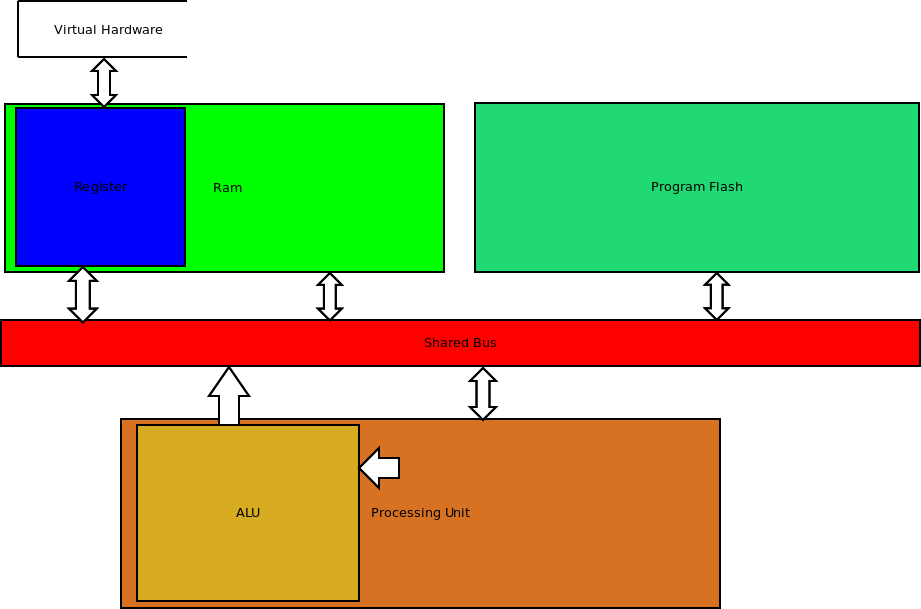
\includegraphics[width=\linewidth]{bloecke.png}
\caption[Blockdiagramm]{Blockdiagramm der Py Register Machine}
\label{fig:bloecke}
\end{figure}

\section{Module}

Sinnvoll ist die Unterteilung in mehrere Speichermodule, sowie den Prozessor:

\begin{description}
\item[Speicher] Der Speicher oder RAM sollte durch ein Objekt repräsentiert werden, am besten von einer Klasse \textit{Memory} abgeleitet. Bei einer Registerintegration enthält der RAM auch die Register.

\item[Register] Jeder Register sollte als eigenes Objekt repräsentiert werden, das erlaubt die Zuweisung von Spezialfunktionen.

\item[Befelsspeicher] Auch er sollte ein eigenes Objekt sein. Eine Vererbung von einer Klasse \textit{Memory} erlaubt eine kompatible Nutzung zum RAM.

\item[Prozessor] Der Prozessor enthält die anderen Module (eventuell über Umwege). Er hat einen Befehlssatz, mit dem er die Befehle interpretiert.

\item[Rechenwerk] Das Rechenwerk (oder ALU \footnote{Arithmetic Logical Unit} ) wird fast immer  in das Prozessormodul, bzw in dessen Befehlssatz integriert, da eine Aufteilung nicht sinnvoll ist.

\end{description}

Allerdings werden die Register manchmal auch als ein Objekt implementiert, der einzige Unterschied zum RAM besteht dann in den Addressen.

\section{Speicher}

Ein iteressantes Thema über das man allerdings vermutlich Kriege führen kann\footnote{ Man kann über fast Alles in der Informatik Kriege führen.}, ist der Speicherentwurf. Dabei gibt es zum Einen die allgemeine Speicherzellenbreite: Je nach Anwendungstyp ist eine andere Breite angebracht, im Allgemeinen wird allerdings niemand bestreiten, dass 64 bit breite Speicherzellen am sinnvollsten sind\footnote{und es geht los...}. 
Ausnahmen bilden selbstverständliche besondere Rechenmodelle, wie 4 bit Zähler. Zudem muss daran gedacht werden, dass die Registermaschine dann minimal 64 bit addressieren kann, daraus folgt, dass bei ASCII\footnote{Und noch ein Kriegsgrund} codierten Zeichen ganze 56 bit brachliegen\footnote{56 bit sind nicht viel, finde ich.}, andere Codierungen sind dann allerdings sehr einfach um zu setzen.

Zudem ist der Befehlsspeicher ein wichtiger und überlegenswerter Teil des Entwurfs:
Man kann für jeden Teil des Befehls eine eigene Speicherzelle belegen:
\begin{lstlisting}[frame=single]
mov r0 r1
...| 01 | 01 | 02 |...
\end{lstlisting}

eine Alternative ist die bei realen Prozessoren oft genutzte Technik, bei der der Opcode auch noch (zumindest eine) Speicherstellen enthält:

\begin{lstlisting}[frame=single]
mov r0 r1
...| 0101 | 02 |...
\end{lstlisting}

\part{Anhang}

\chapter{Zusätze}
\section{Binäres Rechenmodell}
\label{sec:calc_model}

Das binäre Rechenmodell ist elementar für heutige Computer, es bietet die Möglichkeit nur mit logischen Operatoren 
Ganzzahle zu verrechen. Der einfachste Fall ist die Addition:

\begin{description}

\item[Komplementäre Bits] Ist eine Zahl negativ, so sind alle Bits komplementär zur positiven Zahl ( $ -1 + 1 = 0 $  ), bei einer 5 bit Zahl ist also das 5.Bit das Vorzeichen ( $ 0 = + $):
	$$ 0b00001 = 1 $$
	$$ 0b11111 = -1 $$
	
\item[Addition] Die Addition kann wie folgt definiert werden: $ x, y $ und $ z $ seien Zahlen, man kann diese Zahlen indizieren, indem man jede binäre Stelle als Element nimmt: $ \mathrm{0b01001_{3}} = 1 ; \mathrm{0b01001_{2}} = 0 $ . Dann ist die Addition zweier Stellen so definiert:
	$$ \mathrm{x_n} = ( \mathrm{y_n} \hat{  } \mathrm{z_n} ) \hat{  } \mathrm{( ( x_{n-1} \& y_{n-1} ) | ( x_{n-1} \& z_{n-1} ) | ( y_{n-1} \& z_{n-1} ) ) } $$ 
Dabei is $ \mathrm{x_{(-1)}} = 0 $ .

Man kann dabei vorteilhaft auch iterativ statt rekursiv rechnen:

	$$ 0b010011 + 0b100101 = ? $$
	erste Stelle:
	$$ 0b1 + 0b1 = 0b0 ( 0b1 merken ) $$
	zweite Stelle:
	$$ 0b1 + 0b0 + 0b1 = 0b0 ( 0b1 merken) $$
	usw:
	$$ 0b0 + 0b1 + 0b1 = 0b0 ( 0b1 merken) $$
	$$ 0b0 + 0b0 + 0b1 = 0b1 $$
	$$ 0b1 + 0b0 + 0b0 = 0b1 $$
	$$ 0b0 + 0b1 + 0b0 = 0b1 $$
	gesamt:
	$$ 0b010011 + 0b100101 = 0b111000 $$

\item[Subtraktion] Da negative Zahlen komplementär sind, wird das Prinzip der Addition angewendet.

\item[Overflow] Das rekursive Prinip zeigt deutlich das Problem des Überlaufs: rechnet man mit 8 bit breiten Zahlen, wird $\mathrm{x_9} $ nicht berücksichtigt. Ergebnisse die größer als 8 bit sind, sind deshalb inkorrekt. Dafür wurde auf realen Maschinen das Überlaufbit ( bei 8 bit ist das $ \mathrm{x_9} $ ) eingeführt, es ermöglicht Prüfung auf arithmetische Fehler, sowie Addition über zwei Register.

\item[ 1 + 1 = 0 ] Das Prinzip des Überlaufs ist bei Zählern oft nützlich: Der 4 bit Zähler zählt immer von 0 bis 15 und beginnt dann wieder bei 0:
	$$ 0b1111 + 0b1 = 0b10000 ; bei 4 bit 0b0000 $$

\end{description}

\part{Copyright}

\copyright Copyright 2015 Daniel Knüttel

Dieses Dokument ist Freie Dokumentation, frei, wie FREIheit.

Sie dürfen Kopien davon machen, es verbreiten oder verändern, solange Sie mich als Autor mit angeben und die Änderungen kennzeichen.

Für den Fall, dass dieses Dokument Fehler enthält, freue ich mich über einen Bericht, scließe eine Haftung für eventuelle Fehler aber aus.

Wenn Sie mit diesen Bedingungen nicht einverstanden sind, dürfen Sie dieses Dokument nicht nutzen.

Um meine und Ihre Rechte zu gewährleisten, steht es unter der GNU Free Documentation License. Sie ist hier einsehbar: \url{http://www.gnu.org/licenses/fdl-1.3.de.html}


\end{document}

